As already stated, it is straightforward for the two basic parts of
the training part to be parallelised. There is a batch of $n_1$
independent objectives functions to be optimised and $n_1$ bounding
boxes to be built. Both tasks can be applied in a parallel utilizing
all the available CPU cores. Our implementation supports
parallelization using the built-in \proglang{Python}
\pkg{multiprocess}. In figure \label{fig:exec_parallel} we observe the
execution times for performing the inference. The parallel version
performs all tasks between 2.5 and 6 times faster compared to the
sequential. Optimisation problems are solved almost 6 times
faster. Sampling is executed 3.5 times faster, whereas evaluating the
posterior and constructing the bounding boxes almost 2.5 times faster.

\begin{figure}[ht]
    \begin{center}
      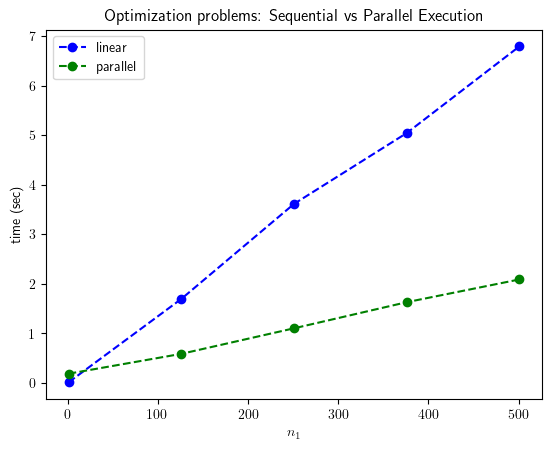
\includegraphics[width=0.35\textwidth]{./latex_files/images/chapter4/solve_problems_parallel.png}
      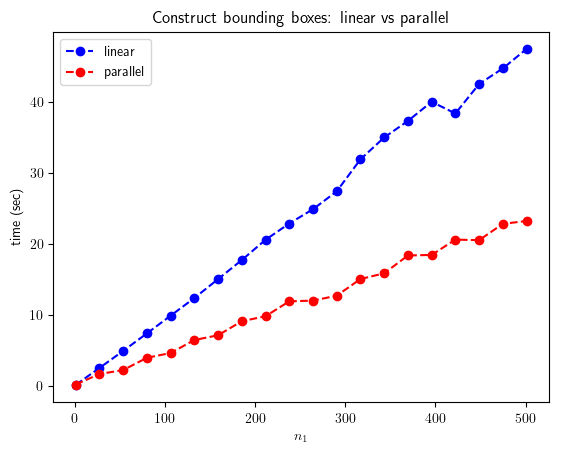
\includegraphics[width=0.35\textwidth]{./latex_files/images/chapter4/estimate_regions_parallel.png}\\
      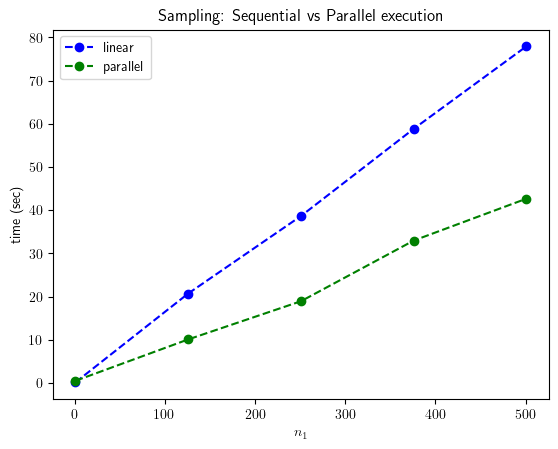
\includegraphics[width=0.35\textwidth]{./latex_files/images/chapter4/sample_parallel.png}
      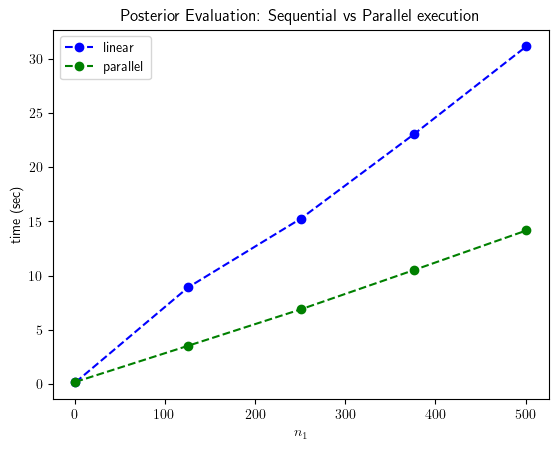
\includegraphics[width=0.35\textwidth]{./latex_files/images/chapter4/eval_post_parallel.png}

    \end{center}
    \caption[Execution time exploiting parallelisation]{In the first
      line, we compare the parallel and sequential execution of the
      training part and at the second line the inference part. At the
      left figure, we measure the execution time for sampling $n_2=50$
      points per region. At the right figure we measure the execution
      time for evaluating the posterior at a batch of $50$ points.}
  \label{fig:exec_parallel}
\end{figure}
